\PassOptionsToPackage{unicode}{hyperref}
\PassOptionsToPackage{hyphens}{url}
\PassOptionsToPackage{table}{xcolor}
\PassOptionsToPackage{centerlast}{caption}
% \PassOptionsToPackage{chapter}{minted}

\documentclass[a4paper,12pt]{article}

% essential packages
% NB: loading mathtools after unicode-math seems to break underbracket
\usepackage{fontspec}
\usepackage[italian]{babel}
\usepackage{mathtools,amssymb,unicode-math}
\setmainfont{Times New Roman}
\setmathfont[Scale=MatchLowercase]{Cambria Math}
\setmonofont[Scale=MatchLowercase]{Iosevka}

% geometry
\usepackage[a4paper]{geometry}
\geometry{hmargin=1cm,vmargin=2cm}

% general packages
\usepackage[final]{microtype}
\usepackage{indentfirst}

\usepackage{float,flafter,caption,subcaption,graphicx,import}
\usepackage{xcolor,xurl}
\usepackage{qrcode}
\graphicspath{{assets/}}

\usepackage{multicol}

\usepackage{enumitem}
\setlist{noitemsep,topsep=0pt}
\setenumerate[1]{label={\arabic*)},ref={(\arabic*)}}
\setenumerate[2]{label={\arabic*.},ref={\arabic*.}}
\setdescription{wide, font=\normalfont}
\newlist{romenumerate}{enumerate}{2}
\setlist[romenumerate,1]{label={\Roman*)},ref={\Roman*}}
\setlist[romenumerate,2]{label={\roman*)},ref={\roman*}}
\newlist{hookdesc}{itemize}{1}
\setlist[hookdesc]{label=$\hookrightarrow$, left=\parindent, beginpenalty=10000}

% Space above and below a float in the middle of the main text
\setlength{\intextsep}{0.25cm}

% float parameters from https://texfaq.org/FAQ-floats
\renewcommand{\topfraction}{.85}
\renewcommand{\bottomfraction}{.7}
\renewcommand{\textfraction}{.15}
\renewcommand{\floatpagefraction}{.66}
\renewcommand{\dbltopfraction}{.66}
\renewcommand{\dblfloatpagefraction}{.66}
\setcounter{topnumber}{9}
\setcounter{bottomnumber}{9}
\setcounter{totalnumber}{20}
\setcounter{dbltopnumber}{9}

% math packages
\usepackage{booktabs,tabularx}
\usepackage{nicematrix}
\usepackage[makeroom]{cancel}
\renewcommand\CancelColor{\color{cadmiumred}}

\usepackage{witharrows}
\WithArrowsOptions{displaystyle,wrap-lines,tikz={-Latex, font={\small}}}
\AtBeginEnvironment{DispWithArrows*}{\ifvmode\noindent\smallskip\fi} % prevent overfull hbox

\NiceMatrixOptions{cell-space-limits = 2pt}
\newenvironment{NiceCases}{\left\lbrace\begin{NiceArray}{*{2}{>{\displaystyle}l}}}{\end{NiceArray}\right.}

\NewDocumentEnvironment{quantities}{m}%
    {\begin{NiceArray}{@{}*{#1}{>{\displaystyle}c@{\,\,\,\,}} @{\!\!\!\!}}}%
    {\end{NiceArray}}

\NewDocumentCommand\mathrnote{m}{\mathrlap{\qquad #1}}
\NewDocumentCommand\con{m}{\mathrnote{\text{con } #1}}

\NewDocumentCommand\hmath{m}{\renewcommand\fboxsep{0pt}\colorbox{cadmiumyellow}{#1}}

% tikz
\usepackage{tikz,tkz-base,tkz-euclide,circuitikz}
\usetikzlibrary{external,positioning,arrows.meta,shapes.geometric,matrix,fit}
\ctikzset{voltage/american minus={}, american voltages, american inductors}
% https://tex.stackexchange.com/a/570721/260531
\tikzexternalize[prefix=figures/]
\tikzexternaldisable
\NewDocumentCommand\ExternalizeThis{m}{\tikzexternalenable\tikzsetnextfilename{#1}}

\tikzset{
% https://tex.stackexchange.com/a/69225/260531
mid arrow/.style={postaction={decorate,decoration={
    markings,
    mark=at position .5 with {\arrow[#1]{Latex}}
}}},
point/.style={inner sep = 1pt, circle, fill},
}

\newlength\CircleArrowLength
\NewDocumentCommand\CircleArrowRight{mm}{
    \setlength\CircleArrowLength{\maxof{\widthof{#2}}{\heightof{#2}}}
    \draw [-Latex, anchor=center, shift=#1]
        node {#2}
        (0,1.2\CircleArrowLength) arc (85:-240:1.2\CircleArrowLength);
}
\NewDocumentCommand\CircleArrowLeft{mm}{
    \setlength\CircleArrowLength{\maxof{\widthof{#2}}{\heightof{#2}}}
    \draw [Latex-, anchor=center, shift=#1]
        node {#2}
        (0,1.2\CircleArrowLength) arc (85:-240:1.2\CircleArrowLength);
}

% table of contents
\usepackage{sectsty,tocloft}
\setcounter{tocdepth}{3}
\allsectionsfont{\bfseries}
\addtolength\cftsecnumwidth{1em}
\addtolength\cftsubsecnumwidth{1em}
\def\cftchapfont{\bfseries}
\renewcommand\cftsecfont{\bfseries}
\renewcommand\cftsubsecfont{\bfseries}
\renewcommand\cftsubsubsecfont{\bfseries}
\addto\captionsitalian{%
    \renewcommand\contentsname{\bfseries Indice}%
    \renewcommand\abstractname{\bfseries Abstract}%
}

% math commands
\usepackage{dsfont}
\newcommand\set[1]{\mathds{#1}}
\newcommand\R{\set{R}}
\newcommand\pinfty{{+\infty}}
\newcommand\minfty{{-\infty}}
\newcommand\seg[1]{\overline{#1}} % segment

\usepackage{derivative}
\NewCommandCopy\pdfrac\pdv

\DeclarePairedDelimiter\pars{\lparen}{\rparen}
\DeclarePairedDelimiter\brak{\lbrack}{\rbrack}
\DeclarePairedDelimiter\brac{\lbrace}{\rbrace}
\DeclarePairedDelimiter\angl{\langle}{\rangle}
\DeclarePairedDelimiter\bars{\lvert}{\rvert}
\DeclarePairedDelimiter\modu{\lVert}{\rVert}

\newcommand\quot[1]{``#1''}

\NewCommandCopy\mono\texttt
\newcommand\code[1]{\colorbox{gray!40}{\textcolor{cadmiumgreen}{\texttt{#1}}}}

\newcommand\vv{\vec{v}}
\newcommand\vu{\vec{u}}
\newcommand\vx{\vec{x}}
\newcommand\vw{\vec{w}}
\newcommand\va{\vec{a}}
\newcommand\vb{\vec{b}}
\newcommand\vzero{\vec{0}}
\newcommand\vr{\vec{r}}
\newcommand\vR{\vec{R}}
\newcommand\vM{\vec{M}}

\newcommand\hv{\hat{v}}
\newcommand\hu{\hat{u}}
\newcommand\he{\hat{e}}
\newcommand\hk{\hat{k}}

\NewDocumentCommand\f{s O{f} m}{#2\IfBooleanTF{#1}{\pars*}{\pars}{#3}}
\newcommand\finv[2][f]{#1^{-1}\pars{#2}}
\newcommand\fp[2][f]{\f[#1']{#2}}
\newcommand\fpp[2][f]{\f[#1'']{#2}}
\NewDocumentCommand\ft{m}{\f[#1]{t}}

\newcommand\g[2][g]{#1\pars{#2}}
\newcommand\gp[2][g]{\f[#1']{#2}}

\newcommand\iu{\mathrm{i}\mkern1mu}
\newcommand\notimplies{\nRightarrow}

\newcommand\md{\mathrm{d}}
\newcommand\dx{\md x}
\newcommand\dy{\md y}
\newcommand\dz{\md z}
\newcommand\dt{\md t}
\newcommand\Dt{\Delta t}

\ifdefined\parallelslant\renewcommand\parallel\parallelslant\fi

\newcommand\qed{\hfill\ensuremath{\square}}

\newcommand\rg{\mathop{\mathrm{rg}}\nolimits}
\newcommand\im{\mathop{\mathrm{Im}}\nolimits}
\renewcommand\hom[2]{\mathop{\mathrm{Hom}}\nolimits\pars{#1, #2}}
\newcommand\sgn{\mathop{\mathrm{sgn}}\nolimits}
\newcommand\trans[1]{#1^{\mathrm{T}}}

\newcommand\existsunique{\mathop{\exists\!!}}

% https://tex.stackexchange.com/a/520268
\newenvironment{system}{\begin{cases}}{\end{cases}}
\NewDocumentEnvironment{LabeledSystem}{O{}}{%
    \begin{NiceArray}{@{}r<{\colon} @{\;\;} \{ >{\displaystyle}l #1 @{}}}{%
    \end{NiceArray}}

\newcommand\hquad{\hspace{0.5em}}

% siunitx
\usepackage{siunitx}
\sisetup{per-mode=symbol, exponent-product=\cdot, inter-unit-product=\cdot}

% text commands
\usepackage{emoji}
\setemojifont{Twemoji Mozilla}
\NewDocumentCommand\sparkle{m}{\emoji{sparkles}#1\emoji{sparkles}}

% colors
\definecolor{darkgreen}{rgb}{0.0, 0.5, 0.0}
\definecolor{chromeyellow}{rgb}{1.0, 0.65, 0.0}
\definecolor{aquamarine}{rgb}{0.5, 1.0, 0.83}
\definecolor{airforceblue}{rgb}{0.36, 0.54, 0.66}
\definecolor{bostonuniversityred}{rgb}{0.8, 0.0, 0.0}
\definecolor{brightgreen}{rgb}{0.4, 1.0, 0.0}
\definecolor{burgundy}{rgb}{0.5, 0.0, 0.13}
\definecolor{cadmiumred}{rgb}{0.89, 0.0, 0.13}
\definecolor{cadmiumgreen}{rgb}{0.0, 0.42, 0.24}
\definecolor{cadmiumorange}{rgb}{0.93, 0.53, 0.18}
\definecolor{cadmiumyellow}{rgb}{1.0, 0.96, 0.0}
\definecolor{darkturquoise}{rgb}{0.0, 0.81, 0.82}
\definecolor{darkviolet}{rgb}{0.58, 0.0, 0.83}

\colorlet{shade}{gray!40}

% quotations
\usepackage{csquotes}
\renewcommand\mkcitation[1]{\par\hfill #1}
\renewcommand\mkccitation[1]{\par\hfill #1}
\SetBlockEnvironment{quotation}

% bibliography
\NewDocumentCommand\SetupBibliography{m}{
    \usepackage[backend=biber, style=numeric]{biblatex}
    \addbibresource{#1}
}

% footnotes
\renewcommand\thefootnote{\Roman{footnote}}

% header
\usepackage{titling,fancyhdr}
\pagestyle{empty}
% \pagestyle{fancy}
% \DeclareDocumentCommand\chaptermark[1]{\markboth{[\thechapter]\ #1}{}}
% \fancyhead{}
% \fancyfoot{}
% \fancyhead[LO,RE]{\bfseries\thepage}
% \fancyhead[C]{\thetitle}
% \fancyhead[LE,RO]{\bfseries\today}
% \fancyfoot[C]{\theauthor}
% \fancyfoot[RO,LE]{\bfseries\leftmark}
% \fancyfoot[C]{\bfseries:)}
% \fancypagestyle{plain}{}

% load package bookmark & hyperref last as per the instructions
\usepackage{bookmark}
\hypersetup{
    colorlinks,
    linkcolor={burgundy},
    citecolor={cadmiumgreen},
    urlcolor={darkturquoise}
}

\AtBeginDocument{%
    % display skip is reset upon \begin{document} so we must set them this way
    \addtolength\belowdisplayshortskip{-3pt}%
    \addtolength\abovedisplayshortskip{-3pt}%
    \addtolength\abovedisplayskip{-5pt}%
    \addtolength\belowdisplayskip{-5pt}%
    \addtolength\belowcaptionskip{3pt}%
}

% subfigure with automatic width
% adapted from https://www.reddit.com/r/LaTeX/comments/42suro/automatically_adjusting_width_in_subfigure/czdsgh8/
\newlength\figwidth
\newsavebox\figbox
\NewDocumentCommand\AutoSubcaption{s O{0pt} m m}{%
    \savebox{\figbox}{#4}%
    \settowidth{\figwidth}{\usebox{\figbox}}%
    \addtolength{\figwidth}{#2}%
    \IfBooleanTF#1%
        {\begin{subtable}[t]{\figwidth}\centering\caption{#3}\usebox{\figbox}\end{subtable}}%
        {\begin{subfigure}[t]{\figwidth}\centering\caption{#3}\usebox{\figbox}\end{subfigure}}%
}

% show date of lecture in margin
\usepackage{marginnote}
\renewcommand*\marginfont{\footnotesize\color{darkviolet}}
\NewDocumentCommand\lecturemark{m}{\protect\marginnote{#1}}

% add a non-numbered chapter with correct toc handling
\NewDocumentCommand\UnnumberedChapter{m}{%
\chapter*{#1}%
\markboth{#1}{#1}%
\addcontentsline{toc}{chapter}{#1}%
}

\NewDocumentCommand\SetupMinted{}{
    % \setminted{autogobble,breaklines,breakbytokenanywhere}
    % \usemintedstyle{molokai} % requires pip package pygments-molokai
    % \definecolor{codeBg}{HTML}{1c1c1e}
    % \setminted{bgcolor=codeBg}
    \usepackage{tcolorbox}
    \tcbuselibrary{minted}
    \tcbuselibrary{breakable}
    \tcbset{listing only,breakable,fonttitle=\bfseries,float*=hbtp,width=\textwidth}
}


\usepackage{qrcode}

\SetupMinted{}
\SetupBibliography{relazione.bib}

\NewDocumentCommand{\mail}{m}{\href{mailto:#1}{\texttt{#1}}}

\begin{document}

\twocolumn[{\begin{figure}[H]
        \setlength{\linewidth}{\textwidth}
        \setlength{\hsize}{\textwidth}
        \centering
        \begin{NiceTabular}{r@{}c@{}l}
            \Block{6-1}{\includegraphics[width=15ex]{./assets/logo.png}} & {\Large\bfseries Carroponte smart}                                          & \Block{6-1}{\includegraphics[width=20ex]{dipartimento}} \\
                                                                         & Giuseppe Damiata (\mail{giuseppe.damiata01@community.unipa.it})             &                                                         \\
                                                                         & Vincenzo Mazza (\mail{vincenzoluigi.mazza@community.unipa.it})              &                                                         \\
                                                                         & Nicolò Spingola (\mail{nicolofrancescomaria.spingola@community.unipa.it})   &                                                         \\
                                                                         & Università degli studi di Palermo, Dipartimento di Ingegneria, Hangar\_9    &                                                         \\
                                                                         & Classe L-8 C.d.L.\@ in Ingegneria Cibernetica Meccatronica (A.A.\@ 2022/23) &                                                         \\
        \end{NiceTabular}
\end{figure}}]

\tableofcontents

\begin{abstract}
    Nella presente relazione si descrive il progetto di un carroponte smart, ovvero un carroponte
    completamente automatizzato grazie all'utilizzo sinergico di un PLC Zelio Logic SR3B261BD,
    completo di moduli aggiuntivi SR343XTBD e SR3NET01BD, ed un Arduino MEGA. Il progetto è capace
    di caricare e scaricare container da una nave merce in totale autonomia, con un totale di
    quattro zone di carico (due poste sul porto e due sulla nave). Inoltre, è possibile monitorare
    da remoto e telecontrollare il carroponte grazie ad un sistema SCADA realizzato con il software
    Vijeo Citect ed il protocollo Modbus. \cite{arm2015real}
\end{abstract}

\section{Introduzione e scopo del progetto}

I carriponte sono macchine utilizzate per il sollevamento e lo spostamento di carichi pesanti;
trovano larga applicazione in innumerevoli campi, tra cui le navi merce, cantieri edili e magazzini.
In particolare si è scelto di modellare un carroponte portuale, dato il suo alto potenziale per
l'applicazione dell'automazione industriale: Le zone da cui caricare/scaricare sono praticamente
fisse, ovvero si carica sempre dalla nave al porto e viceversa.
\cite{ren2021design,li2015data}

L'automatizzazione di tali dispositivi rappresenta un grande vantaggio, permettendo di ridurre i
tempi di fermo macchina (incrementando dunque l'efficienza), diminuire i costi a lungo termine e
rendere molto più sicuro l'intero impianto grazie all'eliminazione dell'elemento umano.
\cite{gupta2004simplified}

Nella trattazione successiva andremo a delineare il nostro prototipo di sistema di controllo per un
carroponte portuale, basato (come anticipato) sull'utilizzo di un PLC Zelio Logic SR3B261BD per
l'automatizzazione progressiva di un sistema precedentemente ad-hoc, basato su un Arduino MEGA. Il
basso costo del sopracitato PLC permette ad un impianto già esistente di mantenere le sue funzioni
di base, delegando ad il PLC le mansioni di telecontrollo e monitoraggio, che svolge in maniera
semplice ed affidabile.

\section{Design e componenti}

Nella presente sezione verranno descritte le scelte progettuali effettuate per la realizzazione del
prototipo.

\subsection{Struttura del carroponte}

Per la realizzazione della struttura del prototipo è stata scelta la stampa 3D, in
particolare la cosiddetta tecnica del \emph{Fused Deposition Modeling} (FDM). Essa si basa sulla
deposizione di materiale fuso su un letto di stampa, ed ha avuto per la progettazione le seguenti proprietà desiderabili.
\begin{itemize}
    \item Sicurezza dei materiali: Il progetto è stato stampato interamente in una tipologia di
        polimero detta PLA (acido polilattico), che è biodegradabile e non tossica in quanto
        prodotta dalla fermentazioni di amidi vegetali. Ciò ha permesso perciò la possibilità della
        struttura con delle stampanti casalinghe, in particolare una \emph{Eryone Thinker SE} ed una
        \emph{Wunhao GR2}.
    \item Basso costo: Una bobina di plastica per la stampa ha un costo di intorno
        \qty{15}{\euro\per\kg}, e per la realizzazione del progetto ne è stata utilizzata la maggior
        parte.
    \item Resistenza: Il PLA ha un elevata resistenza, il che previene a monte eventuali flessioni,
        rotture o deformazioni.
    \item Facilità di lavorazione: Il PLA è un materiale molto facile da lavorare, in quanto
        facilmente tagliabile, forabile e verniciabile. Si presta inoltre bene all'accoppiamento di
        molteplici parti, grazie alla sua capacità di essere giunto mediante colla o viti.
    \item Facilità di stampa: Il PLA è un materiale molto facile da stampare, in quanto non richiede
        temperature elevate o altre particolari condizioni di stampa. Ciò è in contrasto a materiali
        come l'ABS (\emph{acrilonitrile-butadiene-stirene}), che richiede un'elevata temperatura di
        stampa (intorno ai \qty{235}{\degreeCelsius} per l'estrusore contro i
        \qty{200}{\degreeCelsius} del PLA, il che può causare l'offgassing di fumi nocivi dei
        materiali che compongono la stampante in sé) e particolari condizioni di umidità, ed inoltre
        rende assolutamente necessaria una enclosure per la stampante onde evitare la dispersione
        nell'ambiente dei gas nocivi prodotti durante il processo di estrusione del materiale fuso.
        Tuttavia, come la maggior parte delle scelte progettuali in ambito ingegneristico, ciò
        consiste in un trade-off: Materiali come l'ABS hanno una elevata resistenza ai raggi
        ultravioletti del sole (che il carroponte subirebbe in caso di utilizzo in un porto reale),
        mentre il PLA diverrebbe fragile e si degraderebbe nel tempo.
\end{itemize}

Per la progettazione del modello è stato utilizzato il software \emph{AutoDesk Fusion 360}, uno dei
programmi più diffusi della AutoDesk per le progettazioni CAD. Esso permette di realizzare modelli
complessi, grazie anche alla sua vasta gamma di plugin. In particolare, grazie al plugin
\emph{Helical Gear Plus}, è stato possibile progettare su misura i vari ingranaggi e cremagliere del
carroponte.

Analizziamo nel dettaglio ora il modello, mostrato nella sua interezza assemblata in
figura~\ref{fig:allproj} o in versione interattiva cliccando/scannerizzando il codice QR in
figura~\ref{fig:qrcode-sketchfab}.
\begin{itemize}
    \item La base inferiore del modello (cfr.\@ figura~\ref{fig:cremabase}) presenta degli slot perimetrali per l'incastro con la base
        intermedia, ed è formata nella restante parte da una cremagliera sulla quale scorre il carroponte.
    \item La base intermedia del modello (cfr.\@ figura~\ref{fig:gearbase}) presenta anch'essa degli
        slot perimetrali per l'incastro con la base inferiore e la base superiore, oltre a due
        binari nei quali scorre il carroponte e due fori per il cablaggio del servomotore presente
        sull'estremità inferiore del carroponte stesso. Durante la coordinazione delle stampe, si è
        rilevata la necessità di stampare questo pezzo in due parti, pertanto sono state aggiunti
        quattro fori per l'accoppiamento di quest'ultime mediante delle viti.
    \item La base superiore del modello (cfr.\@ figura~\ref{fig:upperbase}) presenta ovviamente
        anch'essa degli slot perimetrali per l'incastro con la base intermedia, nonché i binari per
        lo scorrimento del carroponte ed un foro posteriore per il cablaggio.
        Sulla sua superficie superiore si può trovare la nave merci, che ha due tasche per
        l'alloggio dei container e per la loro eventuale rilevazione mediante dei fotoresistori
        posti in appositi fori. Sulla parte subito successiva alla nave, ovvero sul porto, si trovano poi altre due tasche analoghe.
    \item Il carroponte (cfr.\@ figura~\ref{fig:carroponte}) ha la forma di un ferro di cavallo.
        Alla sua estremità inferiore, come anticipato, troviamo un albero di trasmissione che
        permette lo scorrimento lungo la base inferiore grazie a due ingranaggi ed un servomotore in
        esso incastonato. Alla sua estremità superiore troviamo invece due servomotori con
        altrettanti ingranaggi e cremagliere che permettono lo scorrimento del braccio magnetico
        (cfr.\@ figura~\ref{fig:magnetarm}) lungo gli assi Y e Z, il quale ha ad esso incollato un
        elettromagnete controllabile in corrente continua da \qty{12}{\volt}.
\end{itemize}

\begin{figure}[htbp]\centering
    \caption{Una versione interattiva del modello.}\label{fig:qrcode-sketchfab}
    \qrcode{https://sketchfab.com/3d-models/newproj-v24-7dc020bd51c9496aabd9ac63d64e03c6}
\end{figure}

\begin{figure}[!hbtp]\centering
    \caption{Il modello nella sua interezza.}\label{fig:allproj}
    \includegraphics[width=\linewidth]{renders/AllProj.png}
\end{figure}
\begin{figure}[!hbtp]\centering
    \caption{La base inferiore del modello, sostanzialmente ricoperta da una cremagliera.}\label{fig:cremabase}
    \includegraphics[width=\linewidth]{renders/CremaBase.png}
\end{figure}
\begin{figure}[!hbtp]\centering
    \caption{La base intermedia del modello.}\label{fig:gearbase}
    \includegraphics[width=\linewidth]{renders/GearBase.png}
\end{figure}
\begin{figure}[!hbtp]\centering
    \caption{La base superiore del modello, completa di nave e un container.}\label{fig:upperbase}
    \includegraphics[width=\linewidth]{renders/UpperBase-Boat-Container.PNG}
\end{figure}
\begin{figure}[!hbtp]\centering
    \caption{Il braccio che tiene l'elettromagnete.}\label{fig:magnetarm}
    \includegraphics[width=\linewidth]{renders/BraccioMagnete.png}
\end{figure}
\begin{figure}[!hbtp]\centering
    \caption{Il carroponte, completo di braccio, ingranaggi, cremagliere e servomotori.}\label{fig:carroponte}
    \includegraphics[width=\linewidth]{renders/Carroponte.PNG}
\end{figure}

Iniziali versioni del progetto utilizzavano un motore DC senza spazzole per l'asse X, in
combinazione con un sensore ad ultrasuoni per il controllo a catena chiusa della posizione. Tale
scelta si è rivelata tuttavia fallace a causa dell'attrito incontrato in assenza di cremagliere,
pertanto nella seconda revisione del progetto si è scelto il design precedentemente illustrato.

\enlargethispage{3\baselineskip}
I container sono stati anch'essi stampati in 3D, con due aggiunzioni.
\begin{itemize}
    \item Sulla parte superiore di ciascun container è agganciata con del biadesivo una rondella
        metallica che permette l'aggancio con l'elettromagnete. Tale rondella è avvolta da una
        guaina termo-restringente ai fini di prevenire la magnetizzazione per strofinio.
    \item Sulla parte inferiore di ciascun container sono stati aggiunti molteplici strati di nastro
        isolante nero, ai fini di aumentare il grado di occlusione della luce e rendere più
        affidabili le letture delle fotoresistenze.
\end{itemize}

\subsection{Arduino}

La scelta del microcontrollore per il controllo dei servomotori nonché il resto del sistema ad-hoc
del carroponte è ricaduta su un Arduino MEGA 2560 Rev3. Tale dispositivo offre:
\begin{itemize}
    \item 54 input/output digitali, 15 dei quali possono essere utilizzati come output con la
        \emph{pulse-width modulation} (PWM);
    \item 16 input analogici;
    \item un oscillatore da \qty{16}{\mega\hertz}, per un'accurata sincronizzazione di tutti i
        processi tempo-dipendenti,
    \item alimentazione DC regolata a \qty{5}{\volt}.
\end{itemize}
Tutte queste caratteristiche sono desiderabili data l'elevata complessità del sistema di controllo e
la vasta gamma di trasduttori ed attuatori che bisogna leggere e controllare, come verrà descritto
successivamente.

La precedente revisione del progetto faceva uso di un PLC Simatic IOT2020 che svolgeva ambedue i
ruoli, sia quello dell'Arduino che quello del PLC. Per la seconda revisione, si è scelto di passare
ad un'architettura del sistema ibrida viste le limitazioni del dispositivo sopracitato e per meglio
dimostrare la flessibilità di un PLC Zelio ai fini dell'automatizzazione/industrializzazione
graduale di sistemi già esistenti, visto il costo proibitivo di rimpiazzare da zero molti impianti
di controllo già esistenti.

Inoltre, è necessario un Arduino MEGA piuttosto che un dispositivo di taglia inferiore dato il già
citato requisito di un elevato numero di ingressi analogici (come si può vedere nello schema
elettrico in figura~\ref{fig:schema-elettrico}), che ammontano a ben otto (l'Arduino UNO, ad
esempio, ne ha solamente sei).

L'alimentazione del microcontrollore è disaccoppiata da quella del PLC, e può avvenire liberamente
mediante un qualsiasi alimentatore DC dai \num{7} ai \qty{12}{\volt}.

\subsection{PLC}

Per l'integrazione all'interno di una rete industriale, non c'è scelta migliore di un PLC, cioè un
controllore logico programmabile. Il loro elevato grado di affidabilità e sicurezza permette di
monitorare il sistema da remoto anche nei casi in cui il sistema sottostante di moto incontri
problemi.

Per il progetto in questione è stato scelto il PLC della Schneider Electric denominato Zelio Logic
SR3B261BD, grazie al suo basso costo che mantiene comunque tutte le caratteristiche necessarie e
desiderabili da un PLC. Esso opera ad un livello di tensione pari a \qty{24}{\volt} DC ed offre:
\begin{itemize}
    \item 16 ingressi, tutti utilizzabili come ingressi digitali e solo gli ultimi sei utilizzabili
        come ingressi analogici;
    \item 10 uscite a relè;
    \item la possibilità di aggiunzione di molteplici moduli aggiuntivi, data la sua monomodularità espandibile.
\end{itemize}

Per permettere la tanto citata integrazione in una rete industriale, il PLC è stato equipaggiato con
un modulo aggiuntivo SR3NET01BD, che permette la comunicazione mediante il protocollo Modbus. Tale
aspetto verrà approfondito in dettaglio più avanti.

Infine, per una maggiore risoluzione delle letture analogiche e per permettere l'utilizzo di uscite
analogiche, è stato aggiunto anche un modulo SR343XTBD.

\subsection{Componentistica, cablaggio, sensori e attuatori}

Per il cablaggio del sistema si è scelto di utilizzare cavi \emph{jumper} attaccati a breadboard e
perfboard, secondo lo schema elettrico in figura~\ref{fig:schema-elettrico}.

Per la rilevazione di container, si è scelto di utilizzare dei fotoresistori, che sono stati
appositamente saldati e posti nei fori per esse designate all'interno della struttura del
carroponte. Per la lettura, viene collegato all'Arduino un partitore di tensione (mettendo in serie
a ciascuna fotoresistenza un resistore da \qty{220}{\ohm}). Per la lettura del PLC vi è un apposito
collegamento Arduino-PLC che permette di ottenere in maniera più affidabile le informazioni sulla
presenza dei container, per ragioni che verranno spiegate più avanti.

Per il controllo dei servomotori, si è scelto di utilizzare dei servomotori SG90, per le loro
dimensioni miniaturizzate e la loro larga diffusione. Essi sono collegati a e controllati
dall'Arduino, che è in grado di controllare fino a 15 servomotori contemporaneamente. Per la lettura
del PLC vi è nuovamente un apposito collegamento Arduino-PLC, con l'aggiunta di un filtro
passa-basso del primo ordine (ovvero un circuito RC con $R = \qty{220}{\ohm}$ e $C =
\qty{100}{\micro\farad}$ nonché l'approssimazione di un convertitore da digitale ad analogico) per
trasformare l'output PWM dell'Arduino in un livello di tensione.

L'elettromagnete per l'aggancio dei container viene controllato mediante un MOSFET, visto che
l'Arduino eroga solamente \qty{5}{\volt} e \qty{40}{\milli\ampere} per ogni pin, mentre
l'elettromagnete richiede \qty{12}{\volt} ed un maggiore quantitativo di corrente. L'alimentazione
per quest'ultimo può provenire direttamente da una qualsiasi sorgente DC, ma per la prototipazione è
stata scelta una batteria da \qty{9}{\volt} per ragioni di comodità. La lettura dello stato
dell'elettromagnete dal PLC avviene in parallelo al Gate del MOSFET.

Per le comunicazione dal PLC all'Arduino, si è scelto di utilizzare la strategia dei resistori
pull-up: Normalmente, un resistore fa sì che il livello di tensione sia alto, ma quando il PLC vuole
comunicare con l'Arduino, esso chiude un relè abbassa il livello di tensione a massa, e l'Arduino è
in grado di rilevare tale cambiamento.

\begin{figure*}[htbp]\centering
    \caption{Lo schema elettrico del sistema.}\label{fig:schema-elettrico}
    \includegraphics[height=\textheight]{SchemaKiCAD}
\end{figure*}

\section{Sistema di controllo}

Il sistema di controllo è, come anticipato, di duplice natura, cioè basato sulla sinergia tra il PLC
e l'Arduino. Il primo implementa la logica di telecontrollo e telemonitoraggio, comunicando con lo
SCADA mediante il protocollo Modbus; il secondo implementa il controllo locale dei servomotori e dei
fotoresistori. Andiamo ad analizzare in dettaglio entrambi i sistemi.

\subsection{Lato Arduino}

L'Arduino è programmato in C++ mediante l'apposito IDE, ed implementa un algoritmo di controllo
relativamente complesso. I relativi codici sorgenti sono inclusi in allegato alla fine del
documento.

Partiamo dal descrivere, ad alto livello, l'algoritmo di controllo automatico.
\begin{enumerate}
    \item All'accensione del sistema, è necessaria una fase di calibrazione:
        \begin{enumerate}
            \item i motori vengono portati ad una posizione nota, cioè quella in cui il carroponte è
                in posizione di riposo;
            \item per ciascuna fotoresistenza, viene calcolato il valore medio di lettura in un arco
                di due secondi, che corrisponde al valore di luminosità ambientale. Verrà
                considerata la presenza di un container se la lettura scende sotto il
                \qty{35}{\percent} di tale valore.
        \end{enumerate}
    \item Finita la calibrazione, si entra nel loop principale. Nel caso in cui il PLC richieda
        l'attivazione del controllo manuale, si leggono le posizioni e gli stati desiderati delle
        assi e dell'elettromagnete e si seguono gli ordini dati e non si prosegue col controllo automatico.
    \item Per il controllo automatico, viene eseguita due volte la procedura a seguire, considerando
        prima gli spostamenti dal porto alla nave e poi il viceversa:
        \begin{enumerate}
            \item Ciascuna zona aggiorna il proprio stato:
                \begin{itemize}
                    \item Se è presente un container e si era nello stato \texttt{EMPTY}, si passa
                        allo stato \texttt{HAS\_\-CONTAINER\_\-TO\_\-MOVE}. Se lo stato è invece
                        \texttt{MOVED\_TO}, si rimane in tale stato.
                    \item Se non è presente alcun container, si passa sempre allo stato
                        \texttt{EMPTY}.
                \end{itemize}
            \item Si cerca una zona sorgente nello stato \texttt{HAS\_\-CONTAINER\_\-TO\_\-MOVE} ed
                una zona destinazione nello stato \texttt{EMPTY}.
            \item Avviene la sequenza di spostamento, ovvero si aggancia il container nella
                sorgente, si trasporta alla zona di destinazione e si sgancia delicatamente.
            \item Si verifica l'avvenuto spostamento mediante le letture delle fotoresistenze, ed in
                caso di successo si aggiornano lo stato della sorgente e della destinazione
                rispettivamente a \texttt{EMPTY} e \texttt{MOVED\_TO}.
        \end{enumerate}
\end{enumerate}

Alcune sottigliezze sono state elise nella descrizione di alto livello, perciò analizziamole adesso.
\begin{itemize}
    \item Durante la sequenza di spostamento, è fondamentale muovere ciascun asse individualmente
        per garantire la sicurezza e la prevedibilità degli spostamenti. Inoltre, per simulare la
        reale velocità dei movimenti nonché per garantire il corretto accoppiamento
        ingranaggio-cremagliera, i movimenti dei servomotori vengono rallentati deliberatamente
        attraverso appositi cicli e delay. La posizione in tempo reale viene comunicata in PLC
        tramite il sopracitato filtro passa-basso, visto che quest'ultimo non è in grado di
        decifrare gli impulsi PWM dell'Arduino necessari al controllo dei Servo.
    \item Le letture delle fotoresistenze si sono rivelate, in fase di collaudo, particolarmente
        rumorose. Pertanto le letture vengono mediate in un periodo di \qty{500}{\milli\second}
        prima di decretare la rilevazione. Non si è scelto un filtro passa-basso fisico per le
        letture a causa di limitazioni d'inventario dei progettisti. Tale taratura (e conseguente
        filtraggio) non viene comunicata al PLC, bensì la comunicazione avviene un pin
        \quot{fittizio} che l'Arduino fa variare tra \num{0} e \qty{5}{\volt} in base alle sue
        rilevazioni.
\end{itemize}
Per la semplificazione del codice nonché per garantire un corretto funzionamento del tutto, tali
dettagli implementativi sono stati incapsulati all'interno di apposite classi (nel codice,
\texttt{ServoAxis} e \texttt{Zone}), seguendo il paradigma della programmazione ad oggetti.

\subsection{Lato PLC}

Il programma caricato sul PLC, realizzato con il programma ZelioSoft 2 in linguaggio FBD ed
illustrato in figura~\ref{fig:programma-zelio}, è responsabile per tutto il telecontrollo ed il
telemonitoraggio del sistema, ovvero della comunicazione Modbus tra lo SCADA ed il sistema. Le
tabelle a seguire illustrano gli ingressi, le uscite e le configurazioni dei blocchi. Analizziamo
invece il programma.
\begin{itemize}
    \item Le letture analogiche effettuate mediante l'estensione SR343XTBD corrispondono alla
        posizione corrente sugli assi X ed Y, e vengono direttamente mandate a due word Modbus
        (\%MW20 ed \%MW21). Al contrario, due word del Modbus (\%MW16 ed \%MW17) vengono
        direttamente esposte come le uscite analogiche dello stesso modulo aggiuntivo per indicare
        la posizione desiderata in X ed Y.
    \item Per costituire i cinque bit più significativi della word all'indirizzo \%MW23 viene usato
        un blocco CNA. I primi quattro bit consistono del risultato della comparazione della lettura
        di ciascuna fotoresistenza con due soglie (definite, come si può vedere nella
        tabella~\ref{tab:blocchi-plc}, come 0 e 100), mentre il restante bit corrisponde allo stato
        reale dell'elettromagnete.
    \item La lettura della posizione reale in Z, all'ingresso IB, viene mandata direttamente
        all'indirizzo \%MW22.
    \item I tre bit della \%MW19 vengono esposti, grazie ad un blocco CAN, come tre uscite a relè
        del PLC (Q1 fino a Q3) secondo il meccanismo descritto in precedenza dei resistori pull-up.
\end{itemize}

\begin{figure*}[htbp]\centering
    \caption{Il programma caricato nel PLC.}\label{fig:programma-zelio}
    \includegraphics[height=0.95\textheight]{programma-zelio}
\end{figure*}

\begin{table}[htbp]\centering
    \caption{Gli ingressi del PLC.}\label{tab:plc-inputs}
    \begin{tabularx}{\columnwidth}{@{}lcX@{}}\toprule
        \textbf{Input} & \textbf{Simbolo}                                 & \textbf{Funzione}                                 \\ \midrule
        I1             & \includegraphics[width=16px]{input-digitale}     & Lo stato dell'elettromagnete al presente momento. \\
        IB             & \includegraphics[width=16px]{input-analogico}    & La posizione corrente in Z.                       \\
        ID             & \includegraphics[width=16px]{input-analogico}    & Lettura del fotoresistore zona 1.                 \\
        IE             & \includegraphics[width=16px]{input-analogico}    & Lettura del fotoresistore zona 2.                 \\
        IF             & \includegraphics[width=16px]{input-analogico}    & Lettura del fotoresistore zona 3.                 \\
        IG             & \includegraphics[width=16px]{input-analogico}    & Lettura del fotoresistore zona 4.                 \\
        IH XT2         & \includegraphics[width=16px]{input-analogico-xt} & La posizione corrente in X.                       \\
        IJ XT2         & \includegraphics[width=16px]{input-analogico-xt} & La posizione corrente in Y.                       \\
    \bottomrule\end{tabularx}
\end{table}

\begin{table}[htbp]\centering
    \caption{Le uscite (fisiche e non) del PLC.}\label{tab:uscite-plc}
    \begin{tabularx}{\columnwidth}{@{}lcX@{}}\toprule
        \textbf{Output} & \textbf{Simbolo}                              & \textbf{Funzione}                                                                                            \\ \midrule
        Q1              & \includegraphics[width=16px]{output-digitale} & Abilitazione controllo manuale.                                                                              \\
        Q2              & \includegraphics[width=16px]{output-digitale} & Stato desiderato elettromagnete.                                                                             \\
        Q3              & \includegraphics[width=16px]{output-digitale} & Posizione desiderata in Z.                                                                                   \\
        O1 XT1          & \includegraphics[width=16px]{output-scada}    & Posizione corrente in X per SCADA.                                                                           \\
        O2 XT1          & \includegraphics[width=16px]{output-scada}    & Posizione corrente in Y per SCADA.                                                                           \\
        O3 XT1          & \includegraphics[width=16px]{output-scada}    & Posizione corrente in Z per SCADA.                                                                           \\
        O4 XT1          & \includegraphics[width=16px]{output-scada}    & Insieme di bit corrispondenti alla rilevazione delle fotoresistenze e lo stato corrente dell'elettromagnete. \\
    \bottomrule\end{tabularx}
\end{table}

\begin{table}[htbp]\centering
    \caption{Blocchi configurabili del PLC.}\label{tab:blocchi-plc}
    \begin{tabularx}{\columnwidth}{@{}lcX@{}}\toprule
        \textbf{No.} & \textbf{Simbolo}                           & \textbf{Funzione}                                                                    \\ \midrule
        B026         & \includegraphics[width=16px]{comparator}   & Rilevazione Zona 1, OFF tra le due successive costanti numeriche e ON altrimenti.    \\
        B027         & \includegraphics[width=16px]{comparator}   & Rilevazione Zona 2, OFF tra le due successive costanti numeriche e ON altrimenti..   \\
        B028         & \includegraphics[width=16px]{comparator}   & Rilevazione Zona 3, OFF tra le due successive costanti numeriche e ON altrimenti.    \\
        B029         & \includegraphics[width=16px]{comparator}   & Rilevazione Zona 4, OFF tra le due successive costanti numeriche e ON altrimenti.DA. \\
        B030         & \includegraphics[width=16px]{num-constant} & Soglia minima zone (0).                                                              \\
        B031         & \includegraphics[width=16px]{num-constant} & Soglia massima zone (100).                                                           \\
    \bottomrule\end{tabularx}
\end{table}

\enlargethispage{-1\baselineskip}
La scelta del linguaggio di programmazione FBD (anche noto come FUP per i PLC targati Siemens) è
stata a noi obbligata dalla scelta dell'inclusione del modulo aggiuntivo SR3NET01BD, il quale impone
appunto sia la programmazione in FBD che l'utilizzo di un PLC a \qty{24}{\volt}. In assenza di
questa restrizione, i PLC sono programmabili in cinque linguaggi secondo la terza parte dello
standard IEC 61131 (precedentemente noto come IEC 1131), che risale al 1993 e standardizza cinque
linguaggi di programmazione, di cui tre grafici e due testuali \cite{lewis_1998}. I tre linguaggi
grafici seguono un preciso crescendo di complessità/flessibilità.
\begin{enumerate}
    \item Il linguaggio \emph{Ladder Diagram} (LD o KOP per i tedeschi) è il più diffuso nonché il
        più antico, ma anche il più \quot{semplice}. Venne sviluppato inizialmente dall'azienda
        Allen-Bradley per consentire agli elettrotecnici la programmazione dei PLC. Appunto per tale
        motivo è il più simile ai diagrammi circuitali, ovvero alla logica cablata che volle
        sostituire trasponendola nel mondo informatico. Dietro la sua semplicità apparente si
        nasconde una inevitabile complessità, che viene fuori man mano che il programma sul PLC
        cresce.
    \item Per rendere più semplice la gestione di programmi complessi, venne inventata la
        programmazione in \emph{Function Block Diagram} (FBD o FUP). Essi sono più simili a
        diagrammi a blocchi che a diagrammi circuitali, pertanto hanno una curva di apprendimento
        inizialmente più ripida ma in ultima analisi rendono più maneggevole progetti di media/larga
        scala.
    \item Più recentemente, è stato sviluppato il \emph{sequential function chart} (SFC), simile
        alle \emph{reti di Petri}. Tali reti, e quindi l'SFC, sono atte alla modellazione di sistemi
        ad eventi discreti, permettendo la facile implementazioni di macchine/automi a stati finiti.
\end{enumerate}
I due restanti testuali sono la \emph{Instruction List} (IL o AWL), ovvero praticamente la
rappresentazione testuale dell'LD, e lo \emph{Structured Text}, un linguaggio di più alto livello
simile al C++.

\section{Sistema SCADA}

I sistemi SCADA (acronimo dall'inglese \emph{Supervisory Control And Data Acquisition}) sono dei
sistemi informatici distribuiti utilizzati per il controllo e il monitoraggio remoto dei PLC
\cite{daneels_salter,ferrazza,sielco}. Essi si compongono di:
\begin{itemize}
    \item uno o più computer che fungono da interfaccia uomo-macchina e che eseguono le funzioni di
        supervisione, controllo e acquisizione dati;
    \item una serie di unità periferiche (PLC) che si interfacciano direttamente con il processo
        tramite sensori e attuatori;
    \item una rete di comunicazione che assicura lo scambio di informazioni tra i computer e le
        unità periferiche tramite vari mezzi trasmissivi e protocolli.
\end{itemize}
Essi sono parte integrante della piramide CIM (Computer Integrated Manufacturing, cfr.\@
figura~\ref{fig:piramide-cim}), che rappresenta la gerarchia dei livelli informativi di un'impresa
manifatturiera. Nella piramide CIM, i sistemi SCADA si collocano al terzo livello, detto di
supervisione e controllo, e comunicano sia con i livelli inferiori, relativi ai dispositivi di campo
e ai sistemi di controllo locale, sia con i livelli superiori, relativi alla gestione della
produzione e alla pianificazione strategica. Il ruolo dei sistemi SCADA nella piramide CIM è quindi
quello di fornire una visione globale dello stato dei processi industriali, di raccogliere e
archiviare i dati relativi alle prestazioni e agli eventi, di implementare funzioni di controllo
avanzate e di ottimizzazione, e di interfacciarsi con gli altri sistemi informativi dell'impresa.

\begin{figure}[htbp]\centering
    \caption{La piramide CIM.}\label{fig:piramide-cim}
    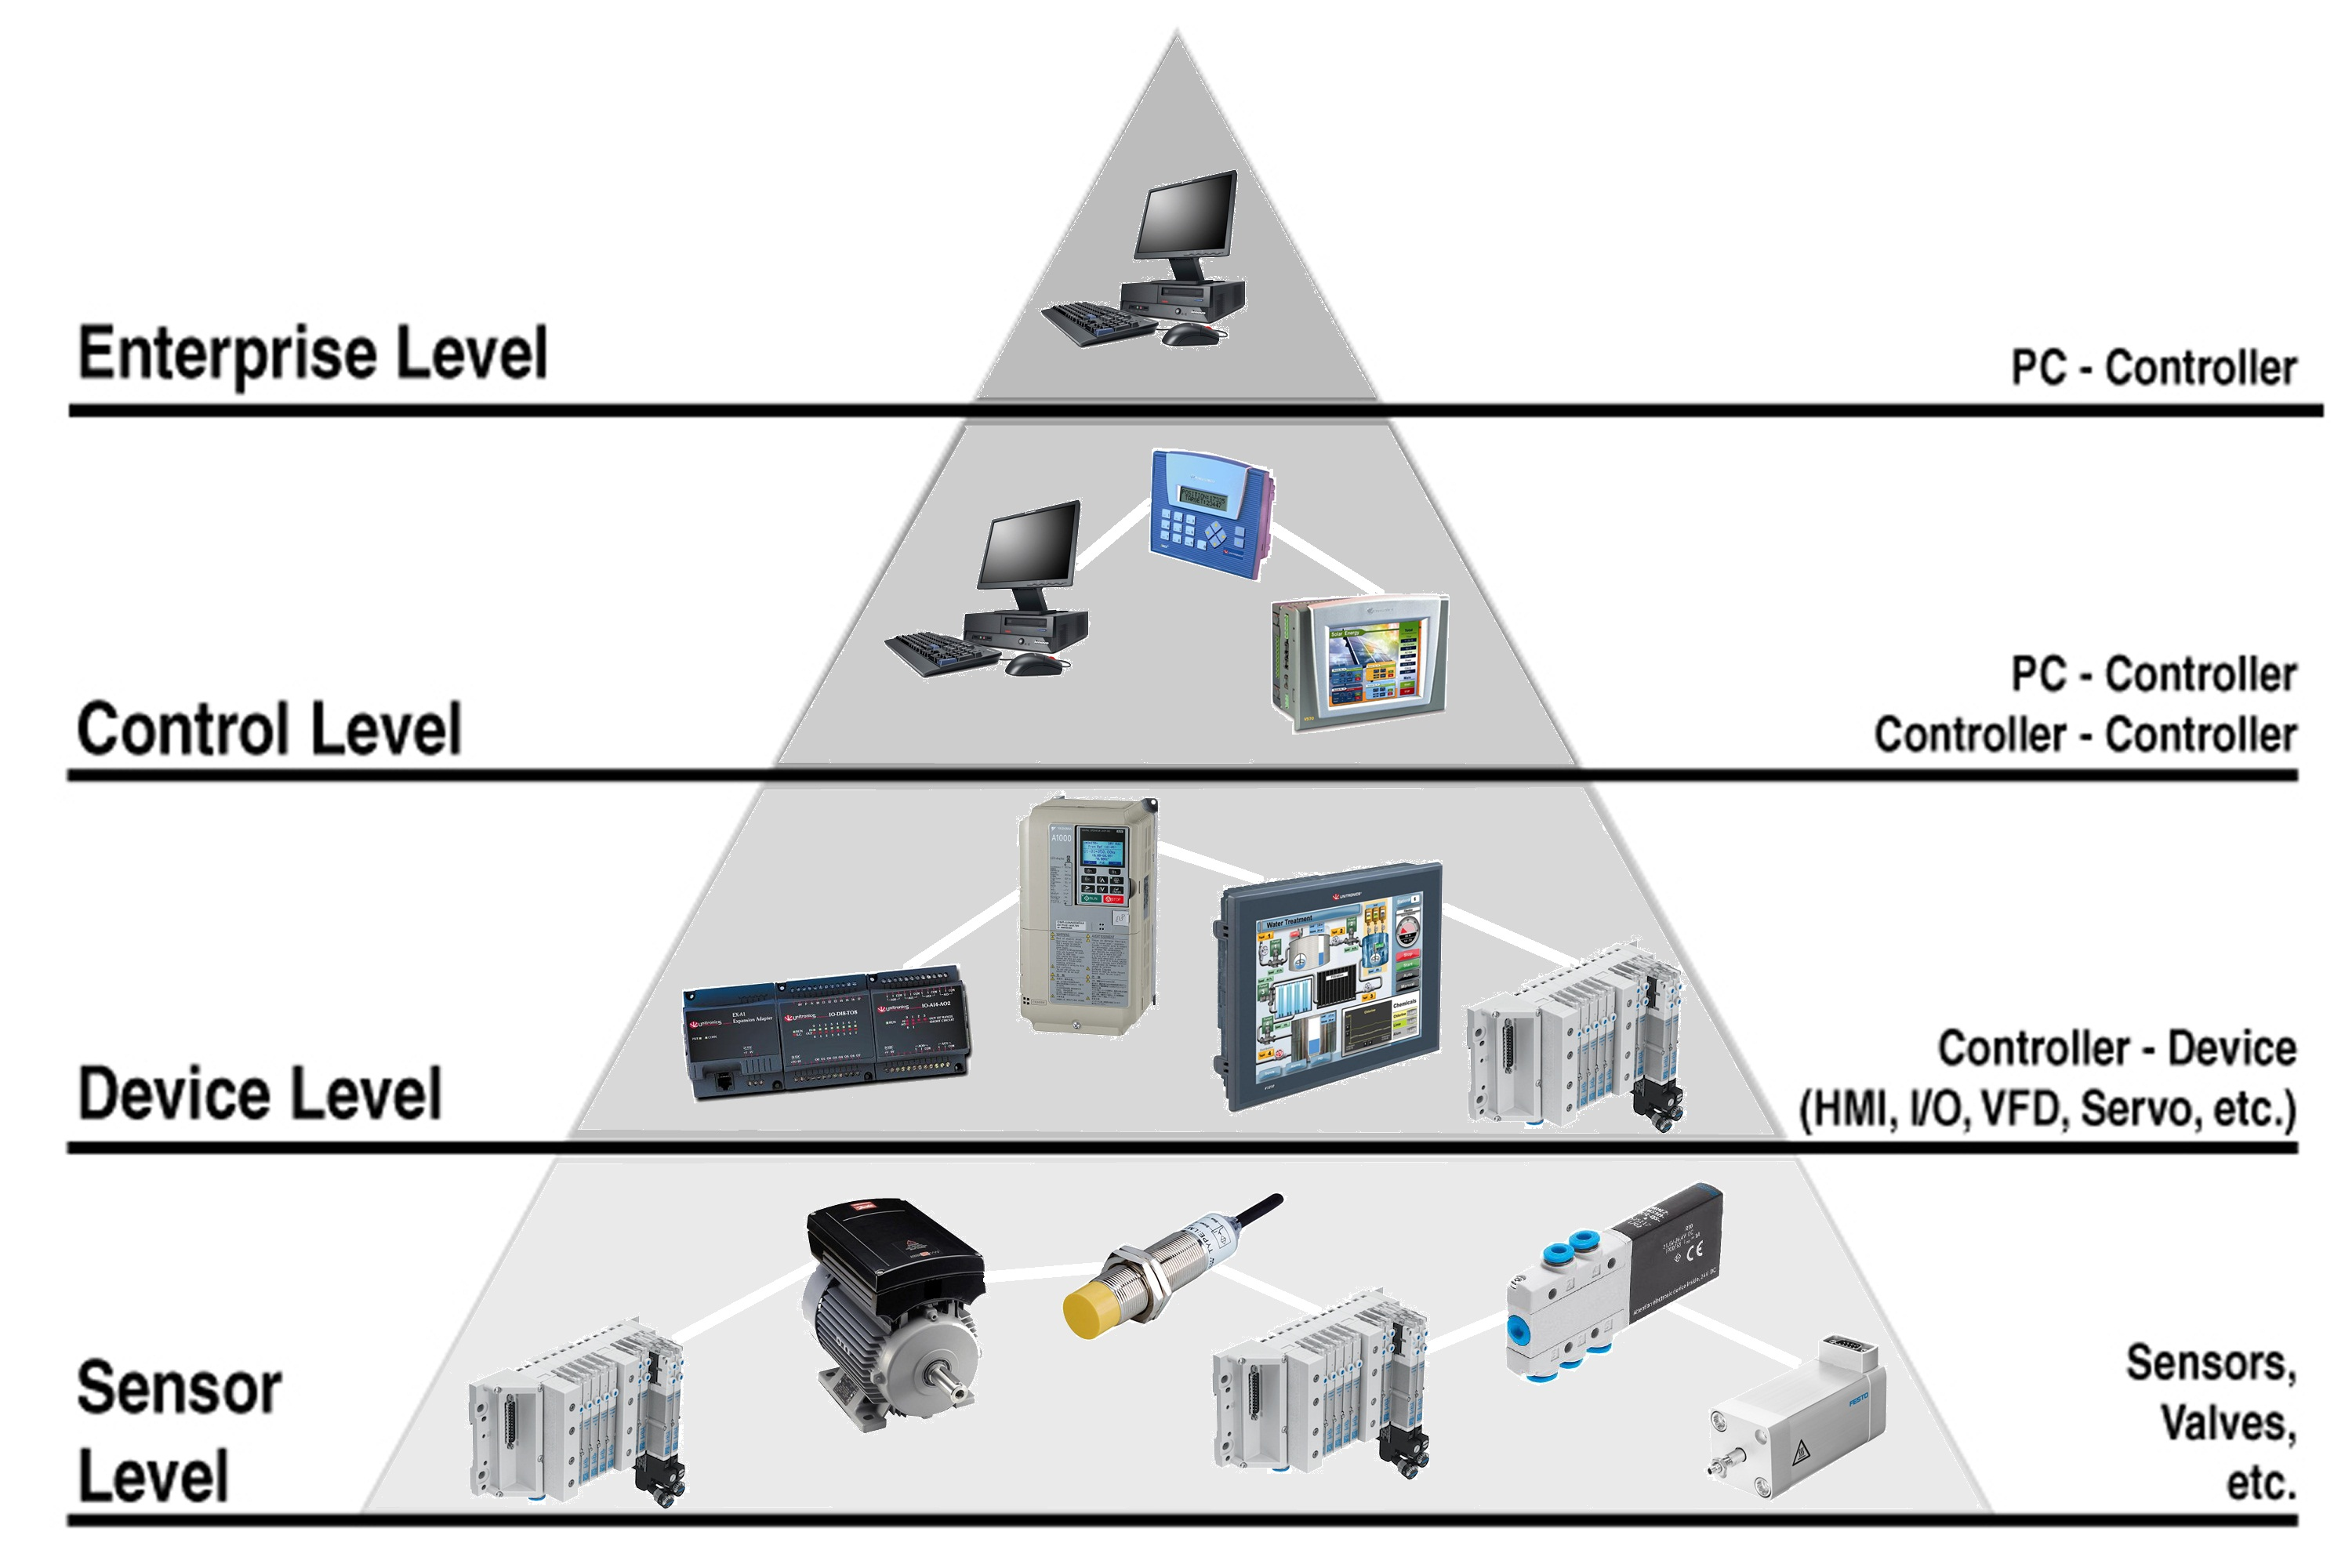
\includegraphics[width=\linewidth]{piramide-cim}
\end{figure}

La comunicazione tra il PLC e lo SCADA avviene mediante il protocollo MODNET, ovvero il protocollo
MODBUS veicolato dal protocollo TCP/IP. Esso dà accesso a 64 bit (impacchettati in quattro interi)
in lettura dal PLC e 64 bit in scrittura dal PLC. Al fine di utilizzarli al meglio, si possono
utilizzare questi interi come valori numerici oppure scinderli nei loro bit costituenti per
trasmettere dati booleani. I quattro interi in lettura sul PLC, ovvero ingressi del programma, sono
indicati come \mono{\%MW16} fino a \mono{\%MW19}. È possibile indicare uno specifico bit aggiungendo
come suffisso la sua posizione a partire dal meno significativo (e.g.\@ \mono{\%MW16.15} è il bit
più significativo di J1). Il discorso è del tutto analogo per gli interi in scrittura dal PLC,
ovvero uscite del programma, che vanno da \mono{\%MW20} a \mono{\%MW23}.

Il sistema SCADA (illustrato in figura~\ref{fig:scada}) è stato realizzato con il software Vijeo
Citect. Esso comunica in tempo reale con il PLC (e quindi con Arduino), e permette di monitorare lo
stato del sistema e di controllarlo manualmente. In particolare è possibile controllare manualmente
le posizioni di tutte e tre le assi, attivare/disattivare il magnete e ottenere le letture di tutte
le zone di carico/scarico. Ciò avviene in tempo reale sia in modalità manuale che in modalità
automatica.

Per configurare la comunicazione è stato utilizzato l'apposito \emph{Express Wizard} presente
all'interno del software. Per la dimostrazione del sistema è stata utilizzata come router un iPhone
attraverso un bridging effettuato con un computer portatile, che presentava come sub-net mask
\mono{255.255.255.40} e gateway \mono{172.20.10.1}, dandoci come possibili scelte per l'IP del PLC
da \mono{172.20.10.2} fino a \mono{172.20.10.14}. È stata selezionato arbitrariamente l'indirizzo
terminante nel numero tredici.

Nel caso di un'implementazione reale sul campo, al posto di un semplice smartphone il nostro sistema
avrebbe seguito un percorso più tradizionale per la comunicazione SCADA-PLC, ovvero il seguente.
\begin{enumerate}
    \item Il PLC legge i segnali di input dai dispositivi sul campo e li memorizza nella sua memoria
        interna.
    \item Il PLC elabora i segnali di input secondo la logica programmata e genera i segnali di
        output ai dispositivi di controllo.
    \item Il modulo aggiuntivo SR3NET01BD trasmette i dati relativi ai segnali di input, output e stato del processo alla
        rete di comunicazione, usando il protocollo Modbus TCP/IP.
    \item Il router/modem riceve i dati dal PLC e li trasmette alla stazione centrale del sistema
        SCADA, usando il protocollo TCP/IP, uno dei protocolli standard più affidabili.
    \item I dispositivi presenti alla stazione di centrale cioè nella sala di comando effettuano
        questo percorso ma in senso inverso.
    \item Il programma SCADA riceve i dati dal PLC e li elabora secondo le funzioni del software,
        visualizzando le informazioni sul processo sull'interfaccia grafica e inviando eventuali
        comandi al PLC.
\end{enumerate}

Un possibile campo di applicazione reale potrebbe poi anche essere quello delle piattaforme
petrolifere offshore, dove ovviamente non si può utilizzare una tradizionale connessione ADSL o in
fibra ottica. In tal caso, sarebbe necessario utilizzare un collegamento satellitare, fornito da
provider come la Starlink, Thuraya o Tuwei.

Avendo costruito la grafica con il \emph{Citect Graphics Editor} (cfr.\@ figura~\ref{fig:scada}), la
programmazione dei comportamenti dei pulsanti nonché degli indicatori è stata realizzata
nell'apposito linguaggio Cicode. I pulsanti permettono di abilitare il controllo manuale, commutare
lo stato dell'elettromagnete e spostare il carroponte lungo l'asse X, andando dal porto alla nave e
viceversa, nonché lungo gli assi Y e Z. Indicatori luminosi mostrano la presenza e l'assenza dei
container nelle quattro zone, nonché la posizione del carroponte e lo stato di abilitazione del
controllo manuale e dell'elettromagnete. Nella tabella~\ref{tab:tags} vengono elencate tutte le tag
utilizzate.

Seguono alcuni dettagli implementativi dello SCADA.
\begin{itemize}
    \item Data l'incertezza delle letture delle posizioni in tempo reale, gli indicatori della
        posizione nave/porto hanno in essi codificata una tolleranza di \ang{10} per elidere gli
        errori di lettura.
    \item La posizione in tempo reale dei tre assi è tarata manualmente in base alle letture di
        tensione in corrispondenza di posizioni note, e poi convertita in gradi mediante una
        semplice proporzione usando l'espressione Cicode che recita
        {\small\mintinline{basic}{IntToStr(TAG/A*B) + "°"}} con $A = \ang{180}$ e $B = \ang{226}$ per
        gli assi X/Y oppure $A = \ang{105}$ e $B = \ang{27}$ per l'asse Z.
\end{itemize}

\begin{figure}[htbp]\centering
    \caption{Il sistema SCADA in funzione.}\label{fig:scada}
    \includegraphics[width=\linewidth]{scada.png}
\end{figure}

\begin{figure}[htbp]\centering
    \caption{Lo SCADA per com'è visto nel Graphics Builder.}\label{fig:scada-builder}
    \includegraphics[width=\linewidth]{graphics-builder.png}
\end{figure}

\begin{figure}[htbp]\centering
    \caption{Un QR code che punta ad una playlist di YouTube illustrativa del funzionamento del carroponte.}\label{fig:qrcode}
    \qrcode{https://www.youtube.com/playlist?list=PLQibPYPJUsXOkAgrr44d6yh03rm6YIBDL}
\end{figure}

\begin{table}[!htbp]\centering
    \caption{Tag di Vijeo Citect.}\label{tab:tags}
    \begin{tabularx}{\columnwidth}{@{}Xcc@{}}\toprule
        \textbf{Nome}                                    & \textbf{Indirizzo} & \textbf{Tipo di dati} \\ \midrule
        {\small Posizione\_\-desiderata\_\-X\_\-J1              } & \%MW16             & INT                   \\
        {\small Posizione\_\-desiderata\_\-Y\_\-J2              } & \%MW17             & INT                   \\
        {\small Enable\_\-controllo\_\-manuale\_\-J4\_\-1       } & \%MW19.0           & DIGITAL               \\
        {\small Stato\_\-desiderato\_\-elettromagnete\_\-J4\_\-2} & \%MW19.1           & DIGITAL               \\
        {\small Posizione\_\-desiderata\_\-Z\_\-J4\_\-3         } & \%MW19.2           & DIGITAL               \\
        {\small Posizione\_\-reale\_\-X\_\-O1                   } & \%MW20             & INT                   \\
        {\small Posizione\_\-reale\_\-Y\_\-O2                   } & \%MW21             & INT                   \\
        {\small Posizione\_\-reale\_\-Z\_\-O3                   } & \%MW22             & INT                   \\
        {\small Zona1\_\-O4\_\-1                                } & \%MW23.0           & DIGITAL               \\
        {\small Zona2\_\-O4\_\-2                                } & \%MW23.1           & DIGITAL               \\
        {\small Zona3\_\-O4\_\-3                                } & \%MW23.2           & DIGITAL               \\
        {\small Zona4\_\-O4\_\-4                                } & \%MW23.3           & DIGITAL               \\
    \bottomrule\end{tabularx}
\end{table}

\section{Conclusioni}

Complessivamente il progetto è da considerarsi un successo: Il controllo automatico funziona come
previsto ed è perfettamente telecontrollabile e telemonitorabile grazie allo SCADA. Il budget è
stato mantenuto ampiamente, grazie anche allo spunto ingegneristico dei progettisti, ed il modello
risultato complessivamente gradevole all'occhio.

In un futuro possibile, tale prototipo potrebbe essere preso come spunto per l'implementazione di un
vero carroponte completamente automatizzato ed integrato in una rete industriale di logistica.

Si ringraziano in primis i progettisti (tra i quali l'autore della presente relazione, che ringrazia
personalmente i suoi compagni per la loro bravura e per la loro compagnia) e soprattutto il
professore Francesco Maria Raimondi per lo spunto di crescita.

% \clearpage
\printbibliography
\clearpage

\tcbinputlisting{title={Lo sketch principale.}, minted language=cpp, listing file=../ProgrammaPrincipale/ProgrammaPrincipale.ino}

\tcbinputlisting{title={Header per il controllo degli assi con servo.}, minted language=cpp, listing file=../ProgrammaPrincipale/ServoAxis.hpp}
\tcbinputlisting{title={File sorgente per il controllo degli assi con servo.}, minted language=cpp, listing file=../ProgrammaPrincipale/ServoAxis.cpp}

\tcbinputlisting{title={Header per la gestione delle zone.}, minted language=cpp, listing file=../ProgrammaPrincipale/Zone.hpp}
\tcbinputlisting{title={File sorgente per la gestione delle zone.}, minted language=cpp, listing file=../ProgrammaPrincipale/Zone.cpp}

\end{document}
% vim: ft=tex
